PocketShelf is an inventory IOS/Android application. Our application consist of many features among which adding item/shelf, search item for each user with Augmented reality experience is the key feature of our application. Diagram below show the overall high level feature of our application.


\begin{figure}[h!]
	\centering
 	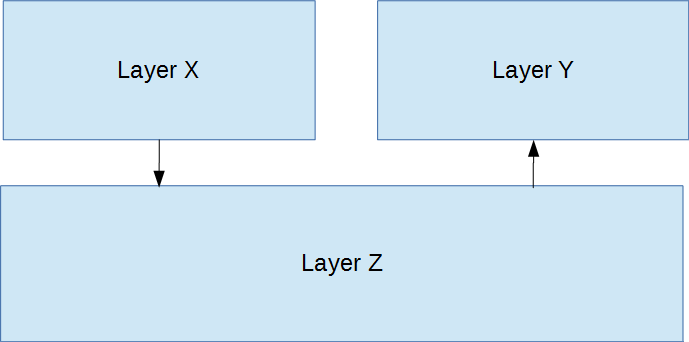
\includegraphics[width=0.60\textwidth]{images/layers}
 \caption{A simple architectural layer diagram}
\end{figure}

\subsection{SignUp}
This is the initial step that is needed to to taken by the user. This layer allows user to create the new account once clicked to signUp in L/R\_UI. In this layer user are required to input the username, email and strong alpha-numeric password. Before any execution the input of the user is validated. Once input is validated, this layer will validate the email, username and password. If the validation and verification is successful, new user is created and all user information is recorded to our database and user is redirected to L/R\_UI.

\subsection{LogIn}
If user clicks LogIn in L/R\_UI, user is redirected to this layer. This layer allow the existing User to login to their account. This layer user to input username and password. Similarly username and password is validated prior to any execution to any query. If valid input are given, layer will logged the user to their respective user home\_UI, if user are registered prior to login.

\subsection{Layer Z Description}
Each layer should be described separately in detail. Descriptions should include the features, functions, critical interfaces and interactions of the layer. The description should clearly define the services that the layer provides. Also include any conventions that your team will use in describing the structure: naming conventions for layers, subsystems, modules, and data flows; interface specifications; how layers and subsystems are defined; etc. 